\section{Results}

% --- SLIDE 1: SUPERVISED BASELINES (TABELAS 6, 7, 8) ---

\subsection{Traditional Regime}

\begin{frame}{Traditional Regime}
    DL models (Transformers and Mamba) consistently outperform SL models with 70\% of labels without pretraining.

    \vspace{0.2cm}

    \begin{table}[h]
        \centering
        \resizebox{0.9\textwidth}{!}{%
        \begin{tabular}{c|l|ccc}
        \hline
        \textbf{Type} & \textbf{Model} & \textbf{Brazil (F1)} & \textbf{Texas (F1)} & \textbf{California (F1)} \\ \hline
        \multirow{3}{*}{Shallow} & SVM & 77.7\% & 98.8\% & 97.2\% \\
         & Random Forest & 75.0\% & 97.9\% & 95.3\% \\
         & MLP & 79.2\% & 99.1\% & 97.0\% \\ \hline
        \multirow{4}{*}{Deep} & SITS-CNN & 83.8\% & 99.5\% & \textbf{98.2\%} \\
         & SITS-LSTM & 84.6\% & \textbf{99.6\%} & 97.4\% \\
         & SITS-BERT++ & \textbf{85.6\%} & 99.5\% & 97.7\% \\
         & SITS-Mamba & 85.0\% & \textbf{99.6\%} & 97.9\% \\ \hline
        \end{tabular}%
        }
    \end{table}
\end{frame}

% --- SLIDE 3: FEW SHOT REGIMES (FIGURAS 54, 55, 56) ---

\subsection{Few Shot Regime}

\begin{frame}{Few Shot Regime}
    \begin{block}{The Impact of SSL in Data Scarcity}
        MoCo pre-training boosts F1-Scores by up to 40\% compared to random initialization.
    \end{block}

    \vspace{0.2cm}

    \begin{figure}
        \centering
        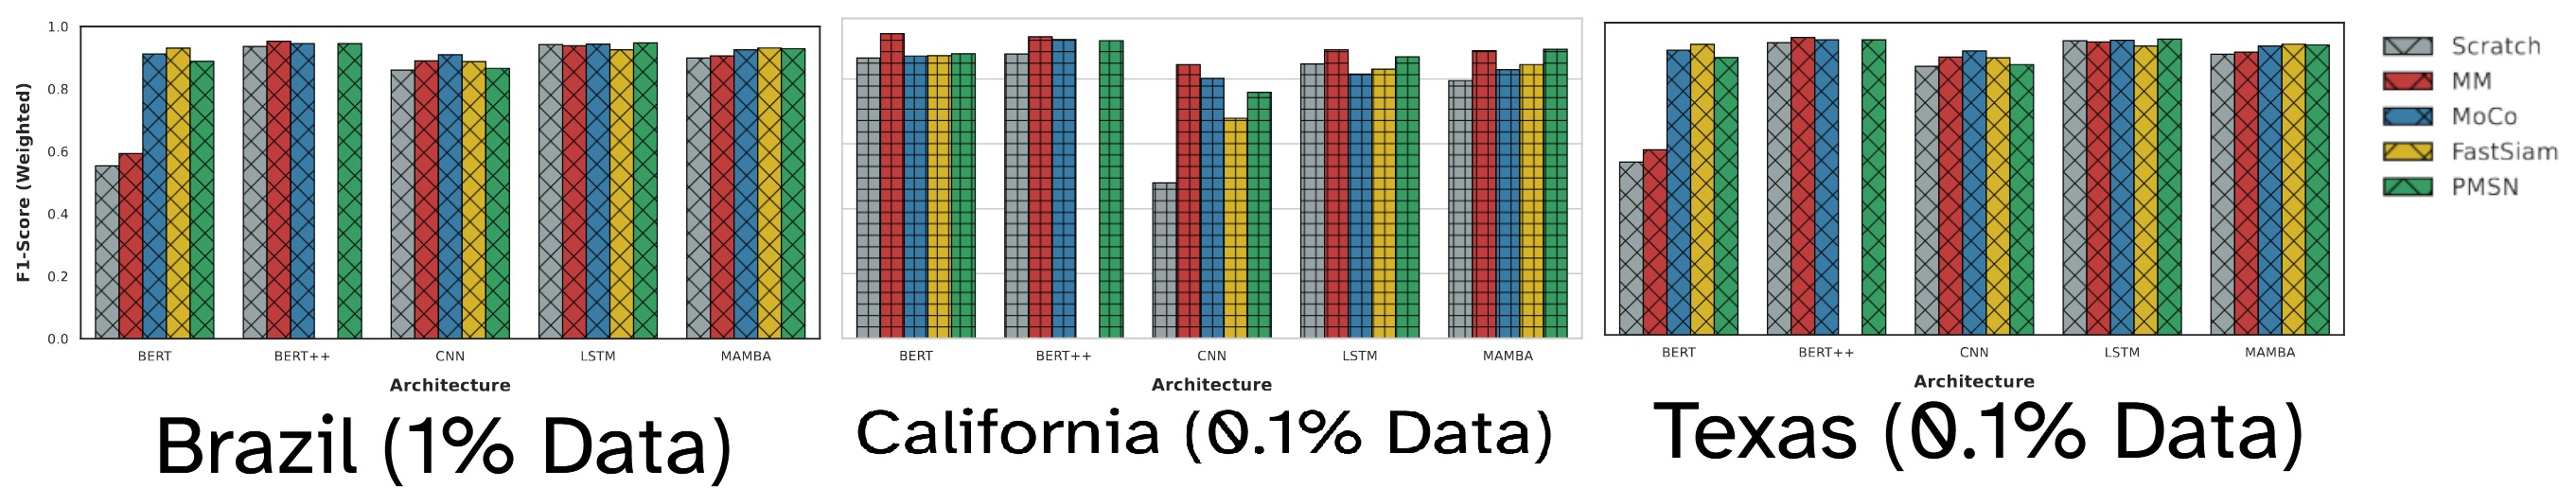
\includegraphics[width=\textwidth, keepaspectratio]{figures_slides/slide_few_shot.jpg}
    \end{figure}
    
\end{frame}

% --- SLIDE 4: DATA SCALING (FIGURAS 57, 58, 59) ---

\begin{frame}{Scaling the Training Data (1\% $\rightarrow$ 10\% $\rightarrow$ 70\%)}
    \begin{block}{Convergence Phenomenon}
        As the availability of labeled data scales to 70\%, the strong supervised signal overrides the SSL initialization, making pre-training less critical. % Architectures like SITS-BERT heavily rely on SSL to avoid poor fitting in few-shot scenarios.
    \end{block}
    
    \vspace{0.2cm}

    \begin{figure}[ht]
        \centering
        % Primeira "coluna" para a Imagem
        \begin{minipage}{0.75\textwidth}
            \centering
            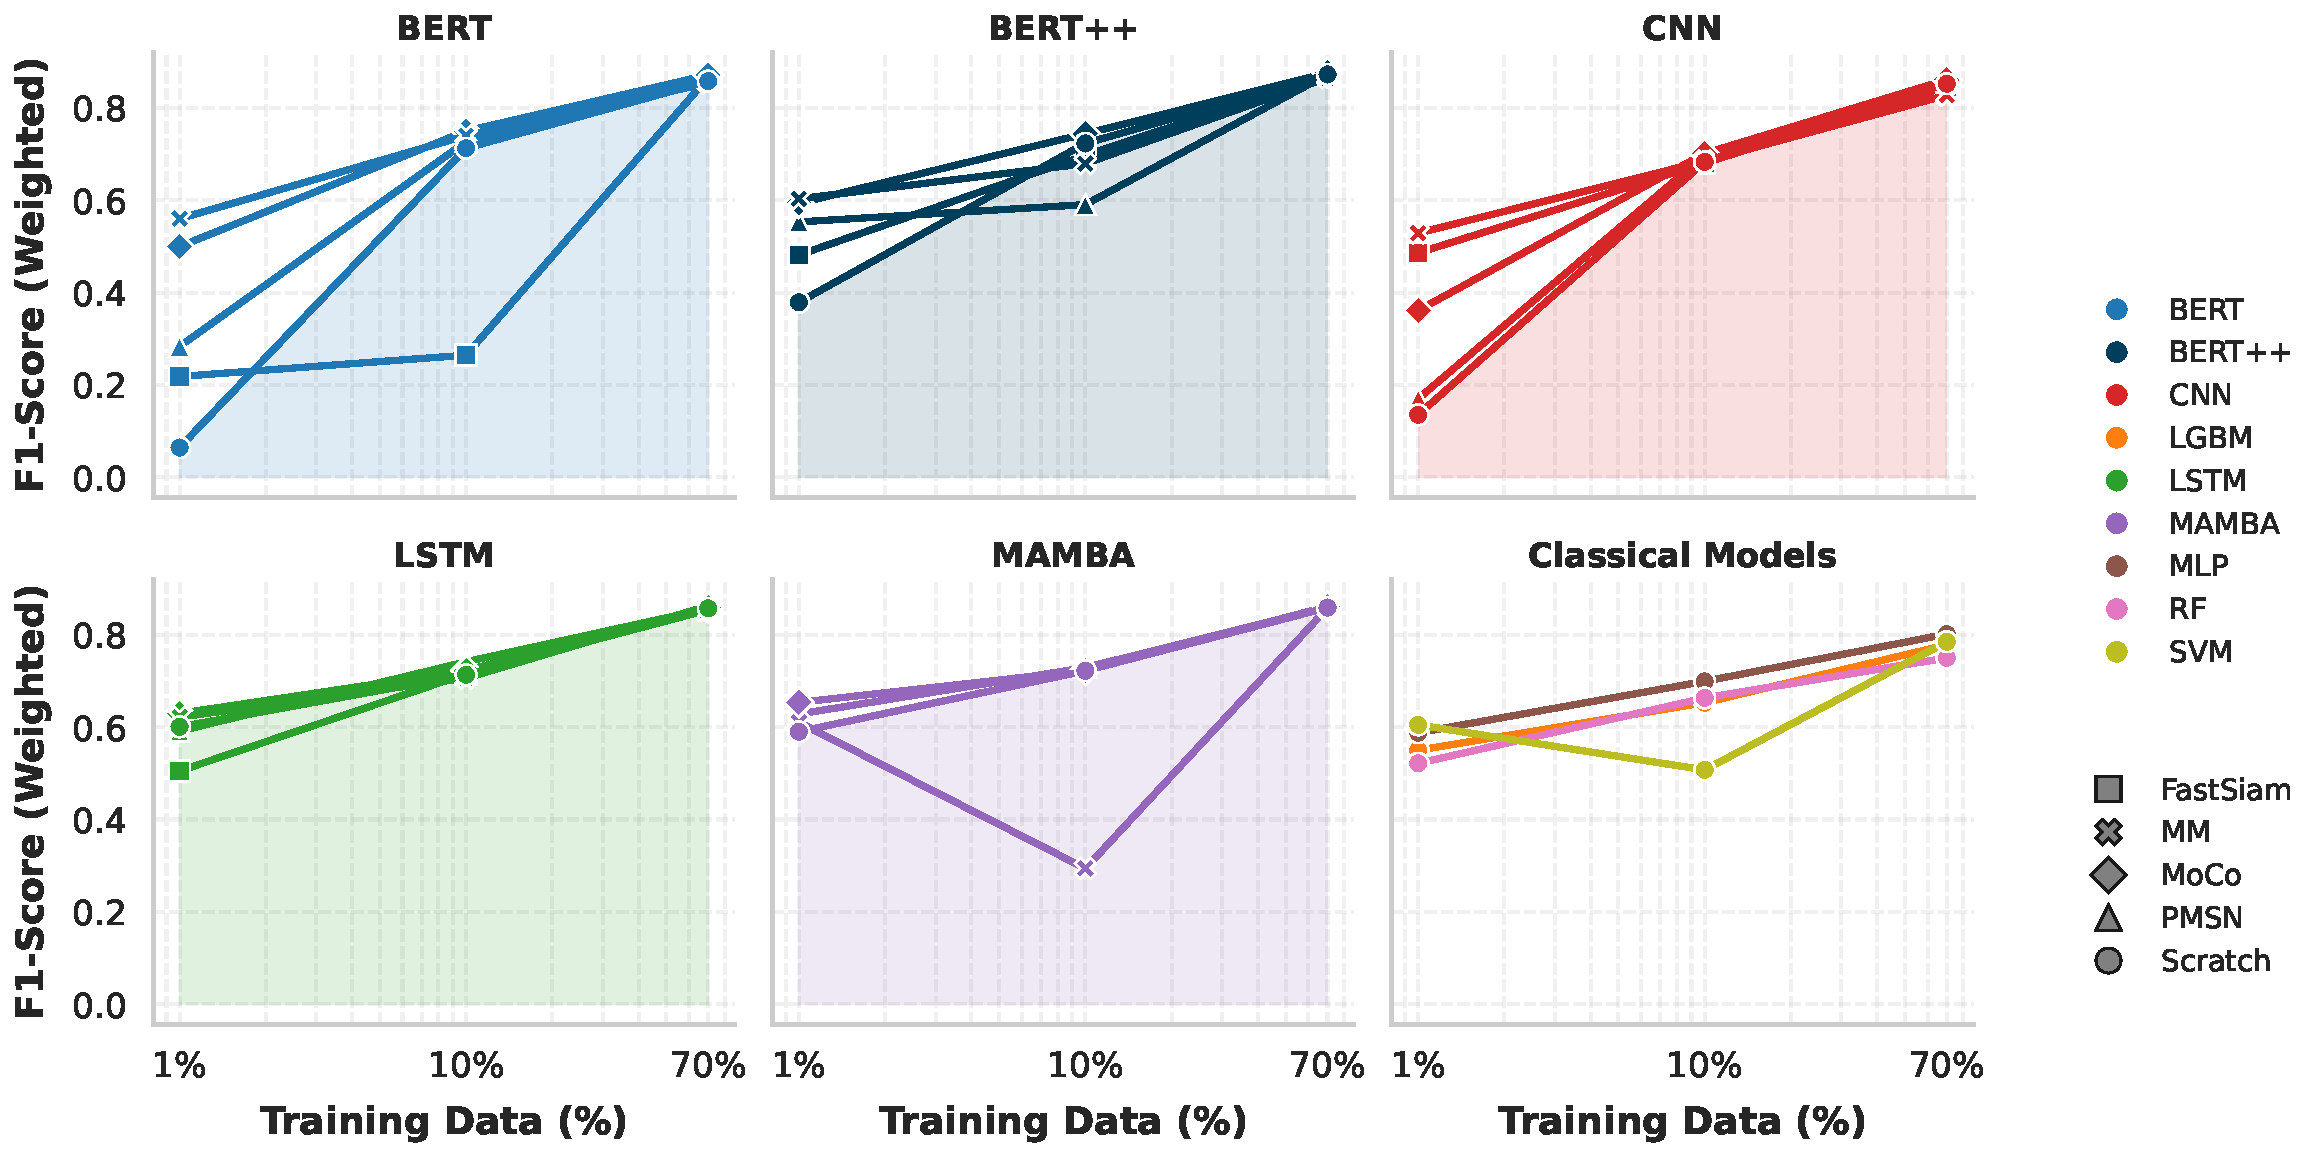
\includegraphics[width=\textwidth, keepaspectratio]{figures/8_results/brazil-finetuning/line_training.pdf}
        \end{minipage}
        \hfill
        \begin{minipage}{0.20\textwidth}
            \caption*{Brazil}
        \end{minipage}
    \end{figure}

\end{frame}

\begin{frame}{Scaling the Training Data (1\% $\rightarrow$ 10\% $\rightarrow$ 70\%)}
    \begin{block}{Convergence Phenomenon}
        The same occurs in the US datasets, although the gain is more marginal.
    \end{block}
    
    \vspace{0.2cm}

    \begin{figure}[ht]
        \centering
        % Primeira "coluna" para a Imagem
        \begin{minipage}{0.75\textwidth}
            \centering
            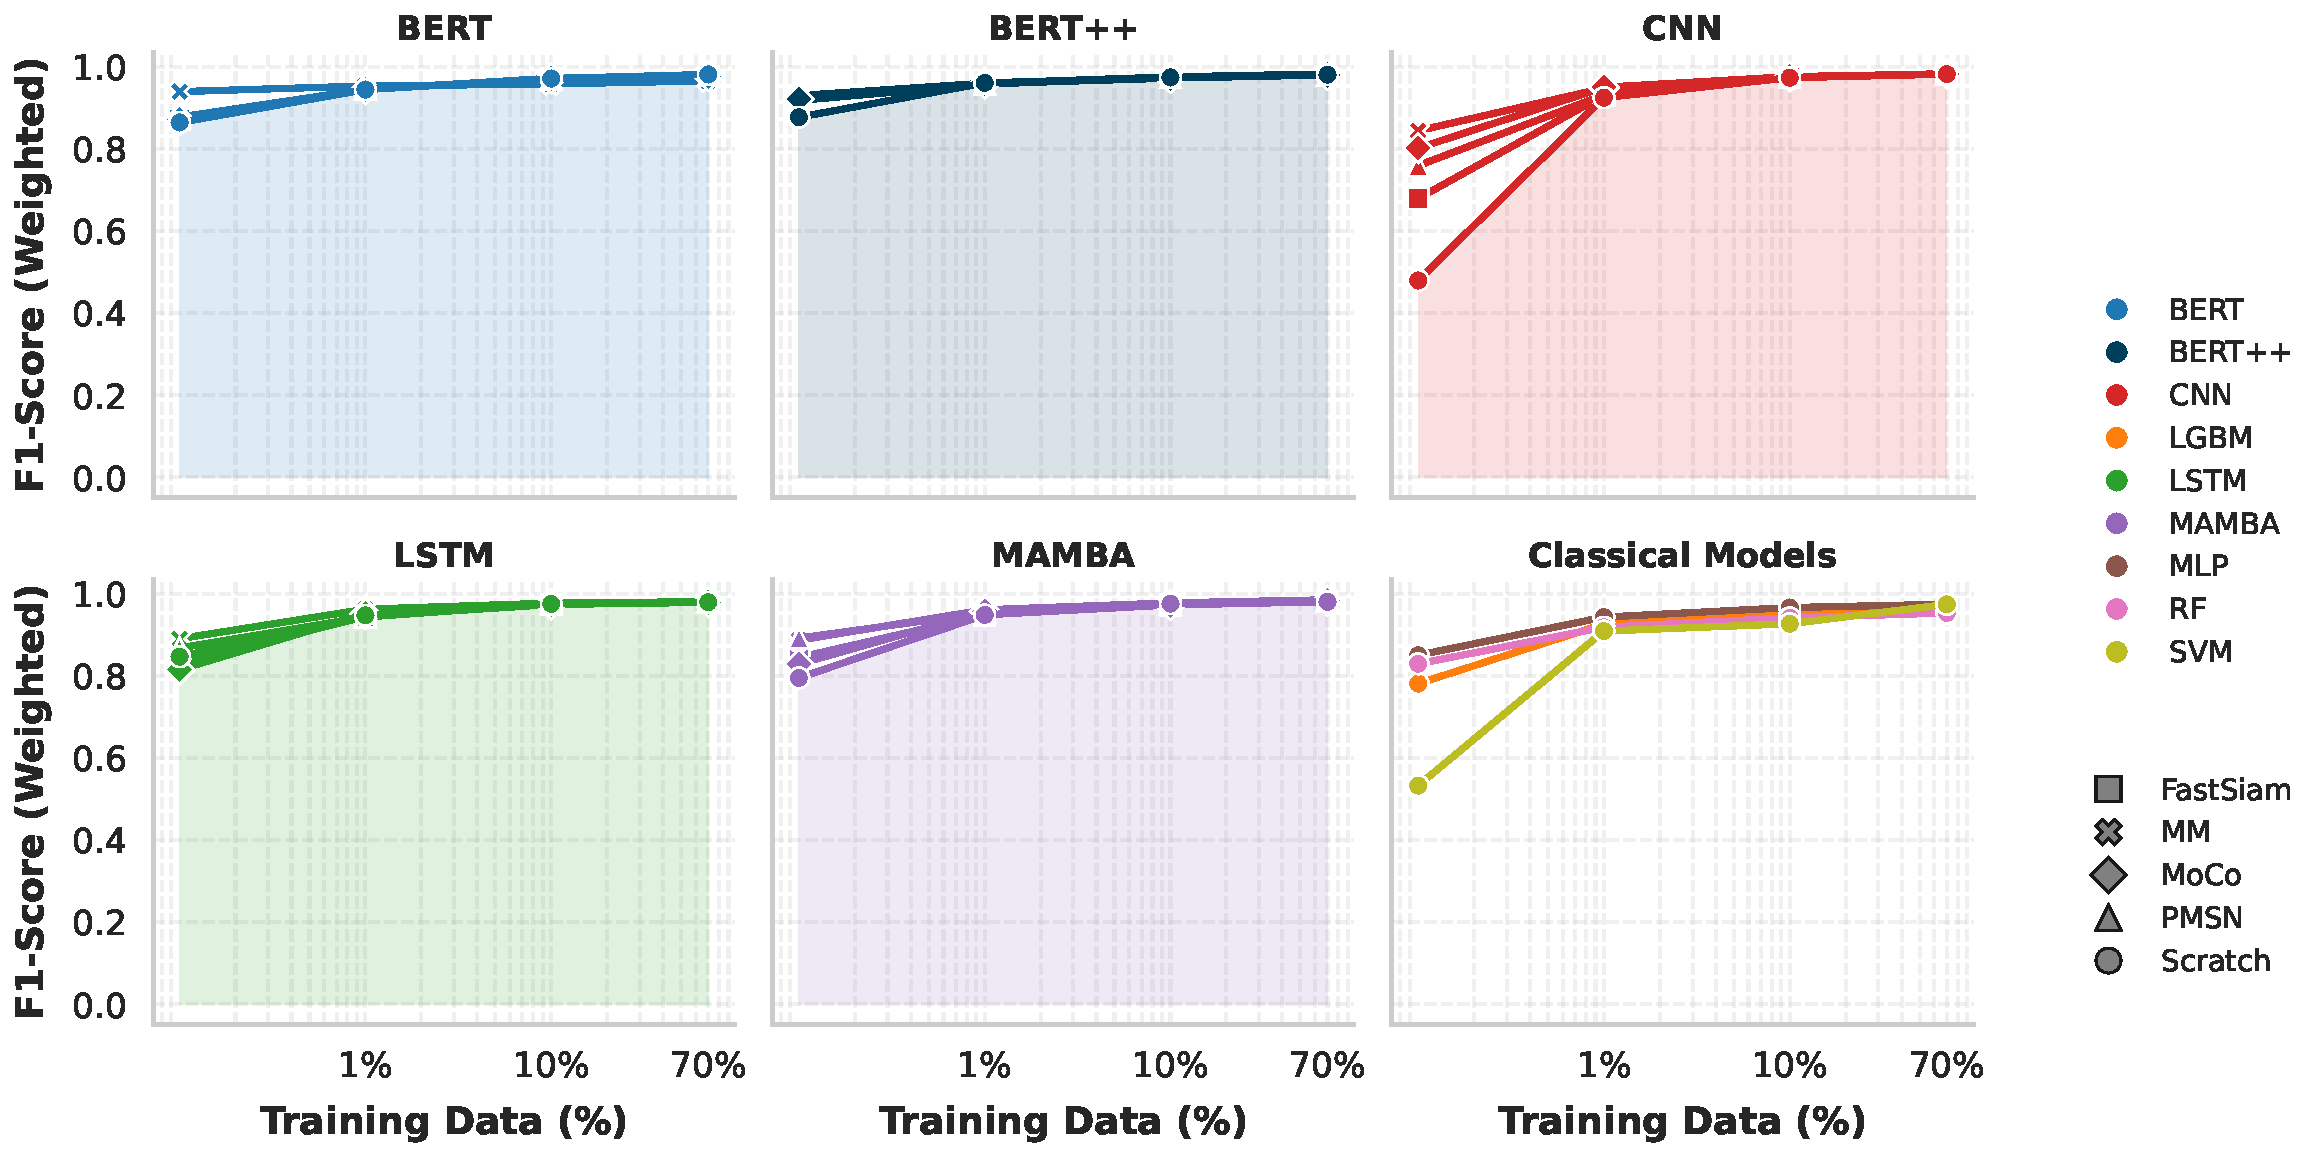
\includegraphics[width=\textwidth, keepaspectratio]{figures/8_results/california-finetuning/line_training.pdf}
        \end{minipage}
        \hfill
        \begin{minipage}{0.20\textwidth}
            \caption*{California}
        \end{minipage}
    \end{figure}

\end{frame}

% --- SLIDE 5: ORDER OVERVIEW (FIGURAS 60, 61, 62) ---

\begin{frame}{Anomaly Detection: The ORDER Method Overview}
    \begin{block}{Rebutting Classification Errors}
        Removing 5\% to 8\% of anomalies in Brazil raised the F1-Score from $\sim84\%$ to $\sim88\%$. In high-accuracy US regimes, ORDER acts remove far fewer samples. %safely and conservatively, targeting genuine label noise without degrading the boundaries.
    \end{block}
    
    \vspace{0.2cm}
    
    \begin{figure}
        \centering
        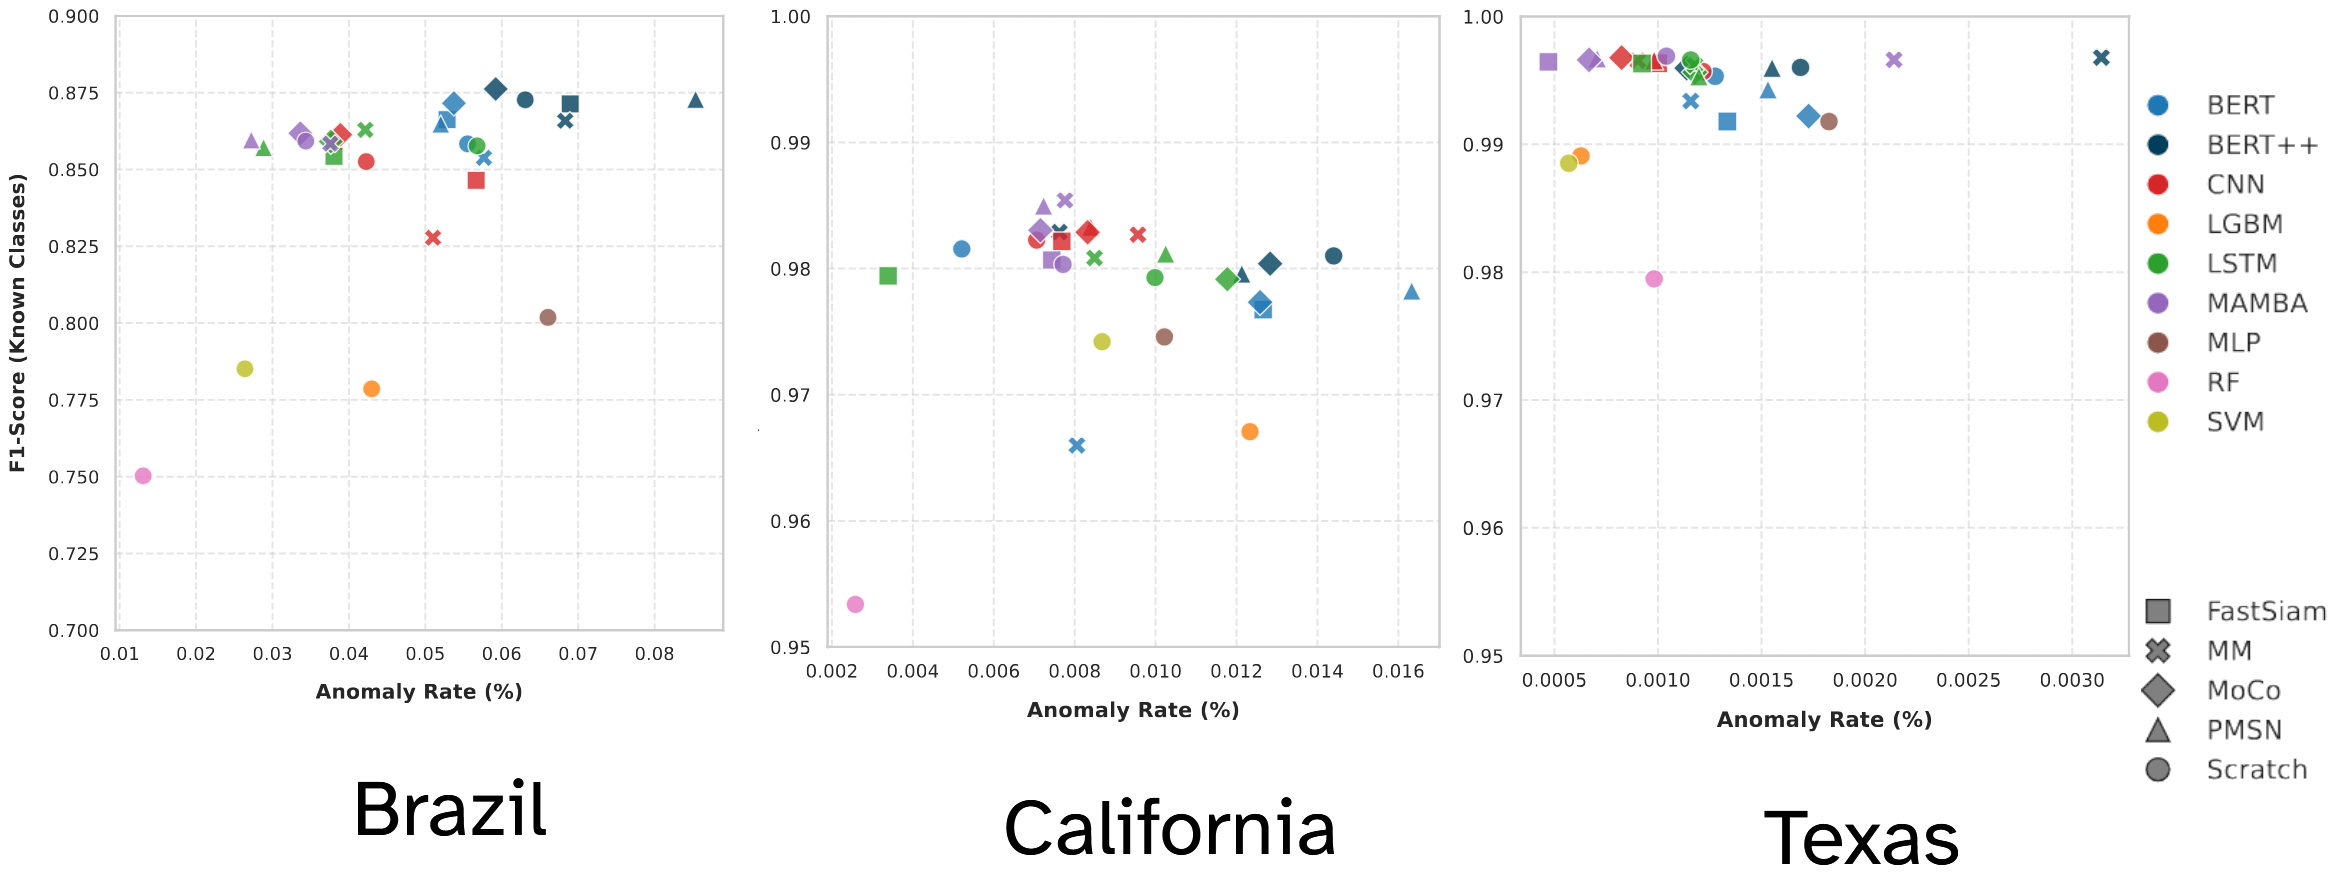
\includegraphics[width=\textwidth, keepaspectratio]{figures_slides/order_slides.jpg}
    \end{figure}

\end{frame}

\subsection{Linear Probing}

\begin{frame}{Self-Supervised Pre-training: Embeddings Quality}
    \begin{block}{Linear Evaluation (KNN F1-Score on Validation Data)}
        Evaluating the latent space via KNN reveals that \textbf{MoCo} generates consistently robust representations across all regions. %\textbf{Masked Modeling (MM)} excels in California, while \textbf{FastSiam} faces collapse issues.% in Transformers/Mamba but performs well with LSTMs.
    \end{block}
    
    \vspace{0.2cm}
    
    \begin{table}[]
        \centering
        \resizebox{0.95\textwidth}{!}{%
        \begin{tabular}{l|ccc}
        \hline
        \textbf{Best Pre-training setups} & \textbf{Brazil (1\%)} & \textbf{Texas (0.1\%)} & \textbf{California (0.1\%)} \\ \hline
        \textbf{MoCo} (Contrastive) & \textbf{63.80\%} (BERT) & \textbf{88.38\%} (Mamba) & 82.98\% (Mamba) \\
        \textbf{MM} (Reconstruction) & 62.18\% (BERT) & 85.25\% (BERT) & \textbf{85.77\%} (LSTM) \\
        \textbf{FastSiam} (Non-Contrastive) & 58.36\% (Mamba) & 87.84\% (LSTM) & 82.38\% (Mamba) \\
        \textbf{PMSN} (Hybrid) & 61.23\% (LSTM) & 88.54\% (BERT++) & 81.45\% (Mamba) \\ \hline
        \end{tabular}%
        }
    \end{table}
\end{frame}

% --- SLIDE 6: BEST RESULT BRAZIL (FIGURAS 63, 64) ---

\subsection{Best Results per Dataset}

\begin{frame}{Best Setup: Brazil Dataset}
    \begin{block}{SITS-BERT++ (MoCo Pre-training)}
        Aside the agricultural complexity of the Brazil dataset, our pipeline achieve far results.% the SITS-BERT++ model with MoCo pre-training establishes a robust baseline despite inherent confusion in challenging classes like Pasture and Temporary Crops..
    \end{block}
    
    \vspace{0.2cm}
    
    \begin{columns}[T]
        \begin{column}{0.48\textwidth}
            \begin{figure}
                \centering
                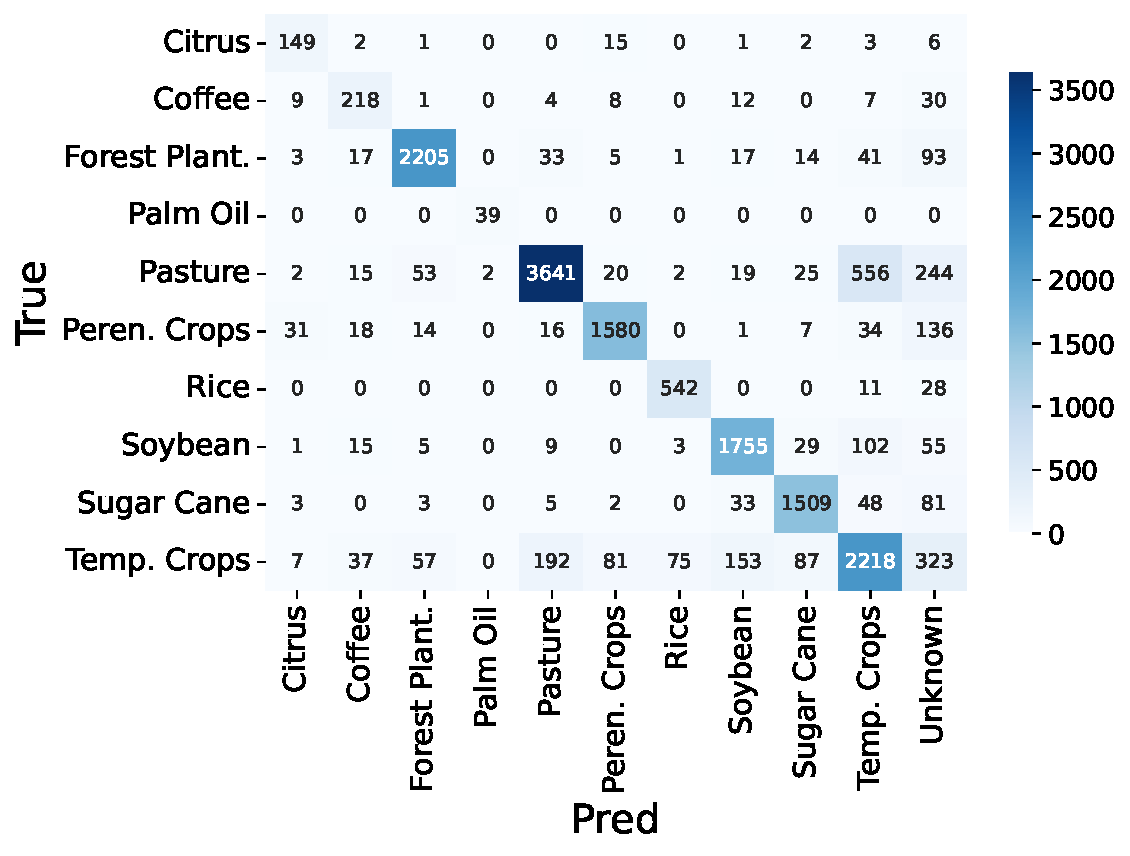
\includegraphics[height=0.45\textheight, width=\textwidth, keepaspectratio]{figures/8_results/brazil-finetuning/BERTPP-70.0-MoCo/class_test_gemmos_matrix.pdf}
                % \caption*{Confusion Matrix}
            \end{figure}
        \end{column}
        \begin{column}{0.52\textwidth}
            \begin{figure}
                \centering
                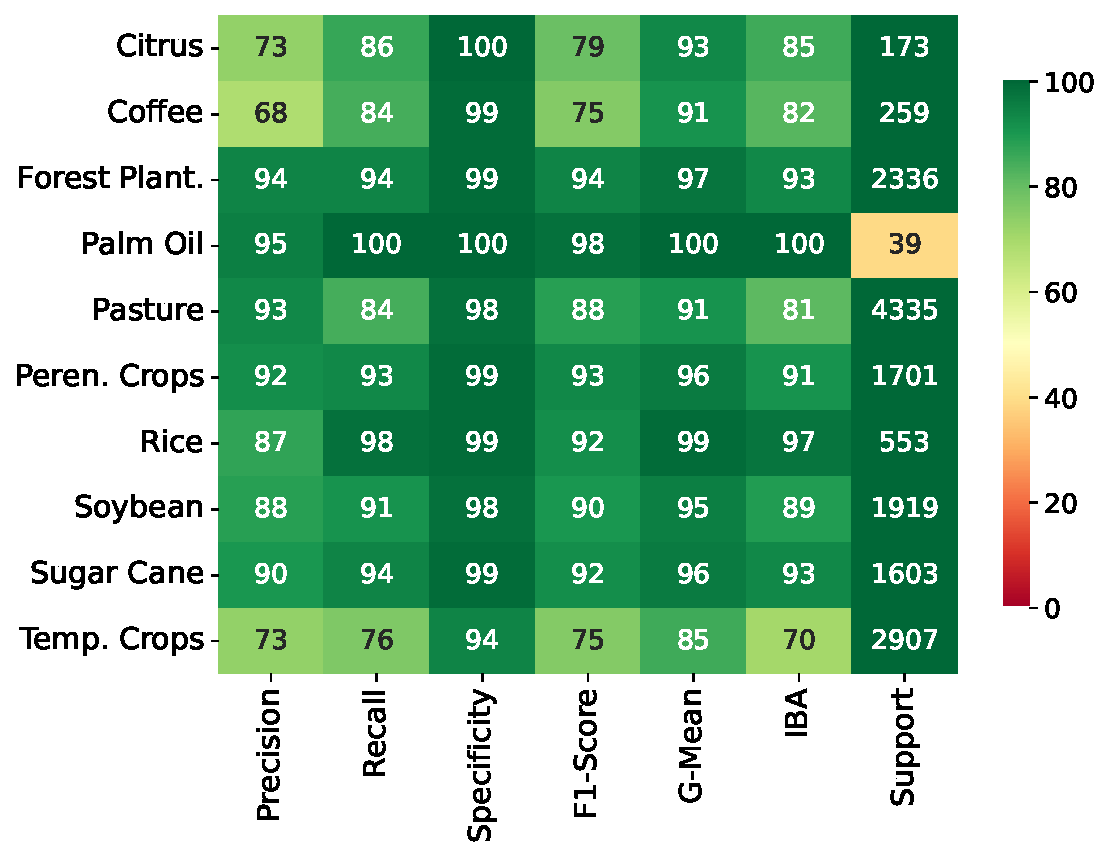
\includegraphics[height=0.45\textheight, width=\textwidth, keepaspectratio]{figures/8_results/brazil-finetuning/BERTPP-70.0-MoCo/class_test_gemmos_report.pdf}
                % \caption*{Confidence Estimation (Log Scale)}
            \end{figure}
        \end{column}
    \end{columns}
\end{frame}

\begin{frame}{Best Setup: Brazil Dataset}
    \begin{block}{SITS-BERT++ (MoCo Pre-training)}
        The proposed ORDER framework achieves a distinct bimodal separation between correct and incorrect predictions for crops like Citrus and Coffee.%, vastly traditional confidence estimators such as ConfidNet and MCP.
    \end{block}
    
    \vspace{0.2cm}
    
    \begin{figure}
        \centering
        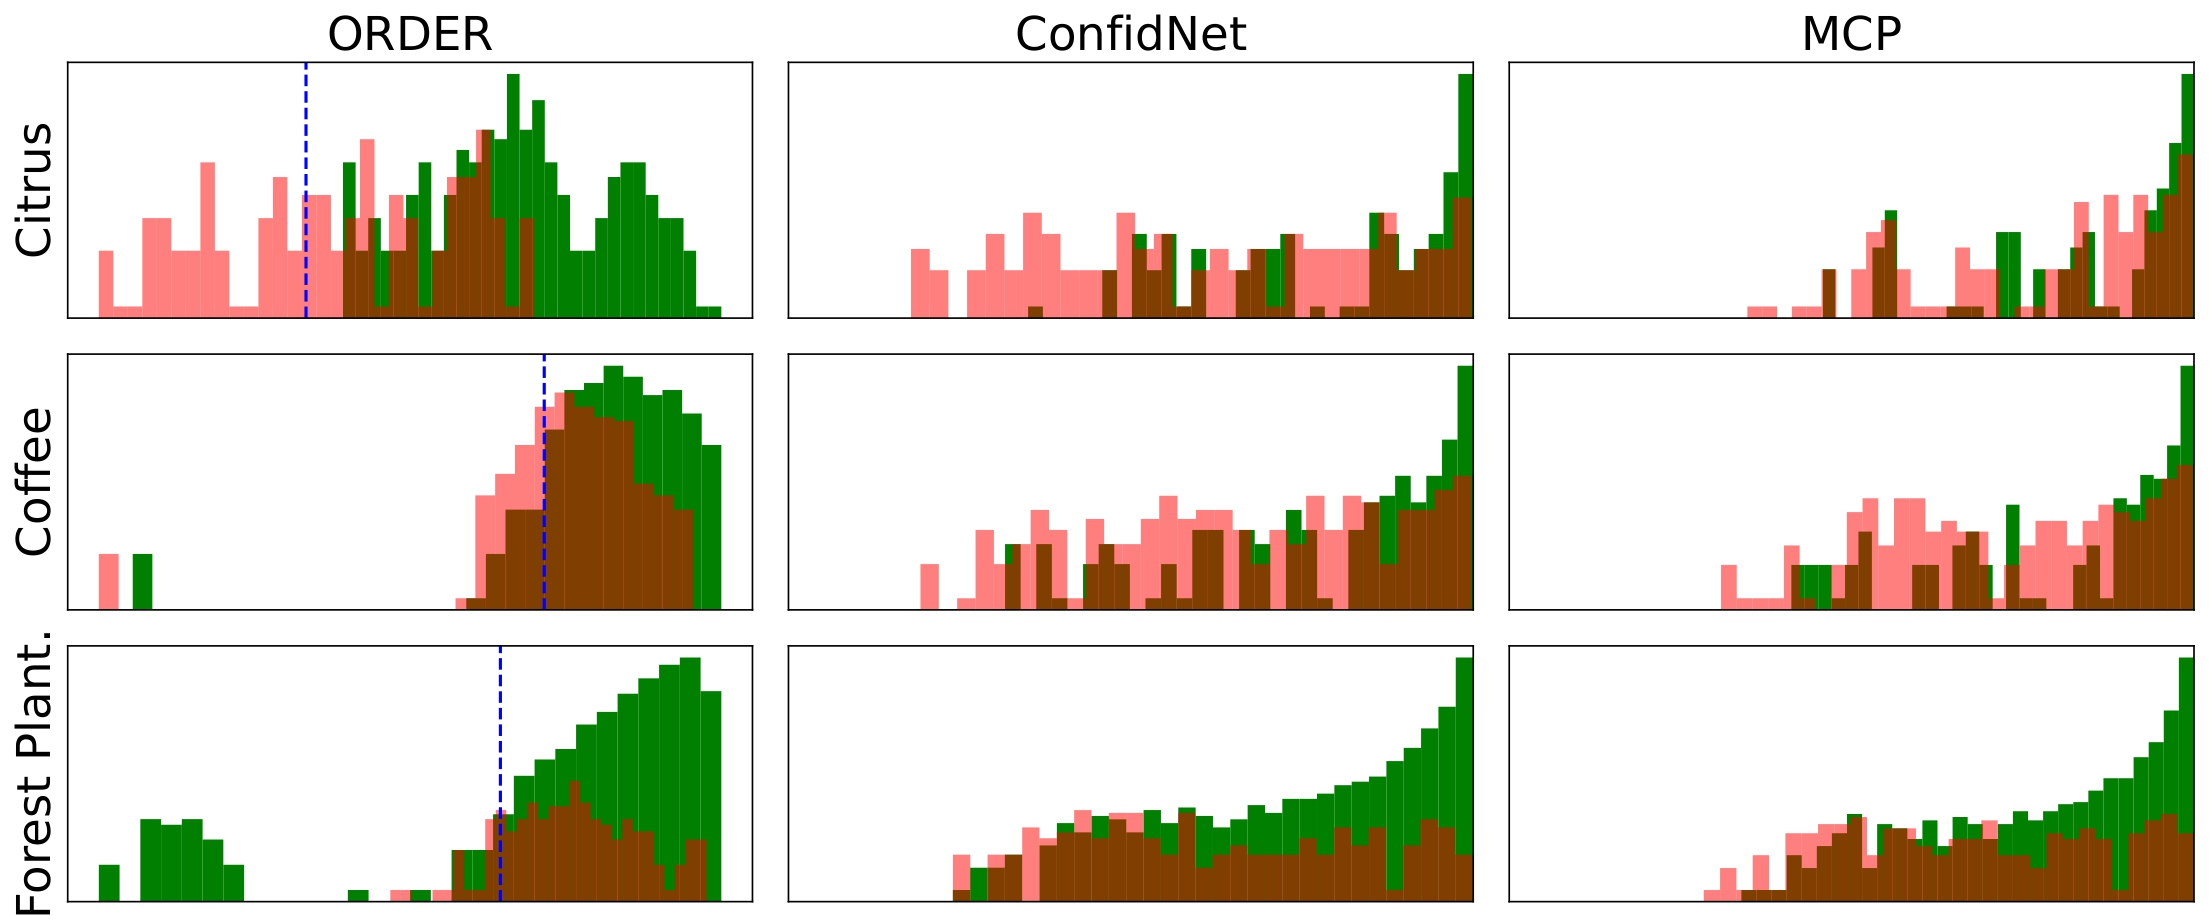
\includegraphics[height=0.41\textheight, width=\textwidth, keepaspectratio]{figures_slides/hist_combined_brasil.jpg}
        % \caption*{Confidence Estimation (Log Scale)}
    \end{figure}

\end{frame}

% --- SLIDE 7: BEST RESULT TEXAS (FIGURAS 65, 66) ---

\begin{frame}{Best Setup: Texas Dataset}
    \begin{block}{SITS-LSTM (FastSiam Pre-training)}
        Transitioning to the Texas dataset, the SITS-LSTM architecture paired with FastSiam pre-training achieves near-perfect classification.%, highlighted by strong diagonal dominance and over 20,000 accurate predictions for Wheat.
    \end{block}
    
    \vspace{0.2cm}
    
    \begin{columns}[T]
        \begin{column}{0.48\textwidth}
            \begin{figure}
                \centering
                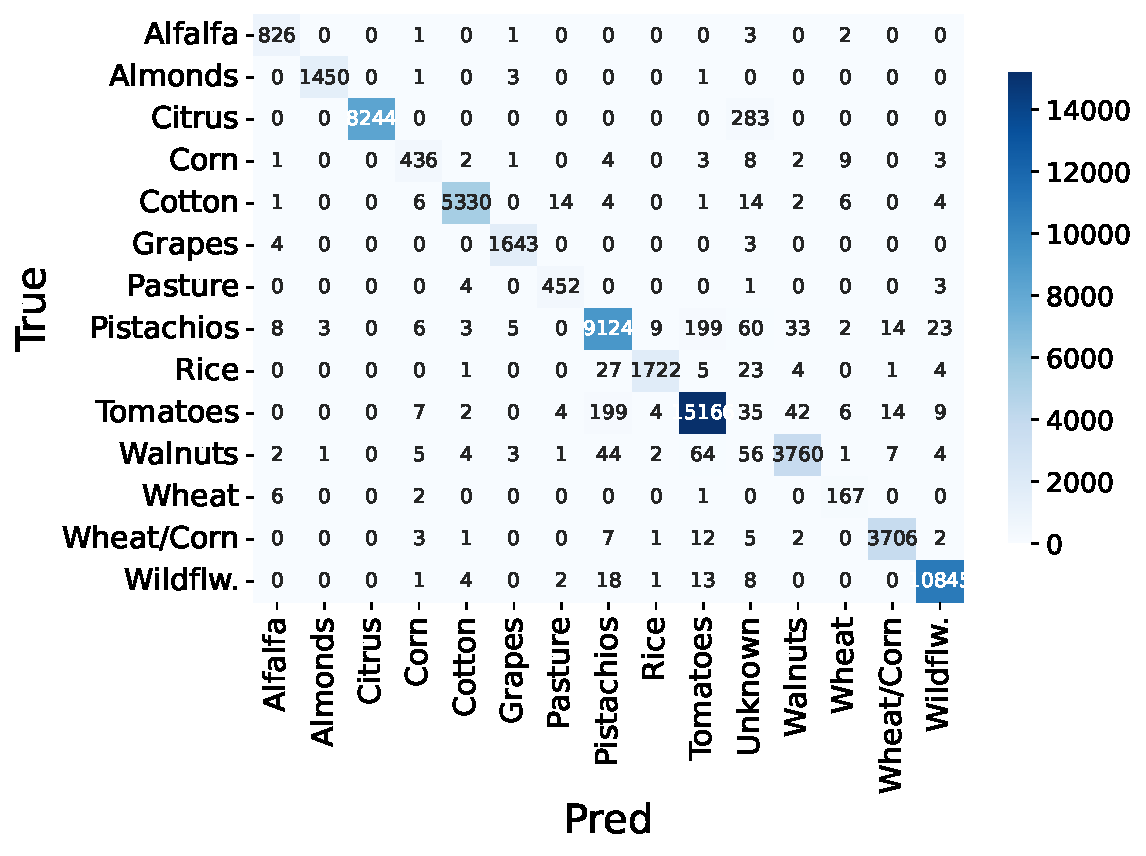
\includegraphics[height=0.45\textheight, width=\textwidth, keepaspectratio]{figures/8_results/california-finetuning/MAMBA-70.0-reconstruct/class_test_gemmos_matrix.pdf}
                % \caption*{Confusion Matrix}
            \end{figure}
        \end{column}
        \begin{column}{0.52\textwidth}
            \begin{figure}
                \centering
                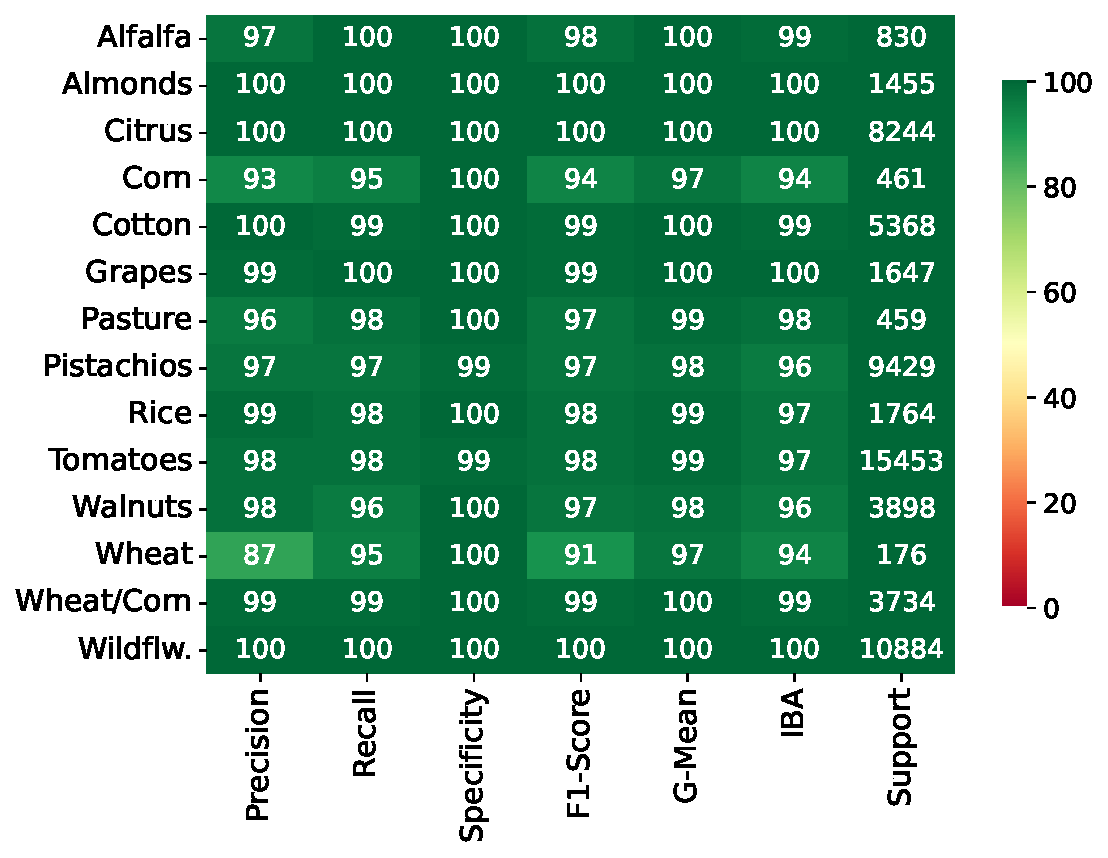
\includegraphics[height=0.45\textheight, width=\textwidth, keepaspectratio]{figures/8_results/california-finetuning/MAMBA-70.0-reconstruct/class_test_gemmos_report.pdf}
                % \caption*{Confidence Estimation (Log Scale)}
            \end{figure}
        \end{column}
    \end{columns}
\end{frame}

\begin{frame}{Best Setup: Texas Dataset}
    \begin{block}{SITS-LSTM (FastSiam Pre-training)}
        Although this exceptionally low error rate challenges standard anomaly visualization, ORDER successfully mitigates the total confidence saturation.% typically observed in baseline methods across classes such as Oats, Cotton, and Corn.
    \end{block}
    
    \vspace{0.2cm}
    
    \begin{figure}
        \centering
        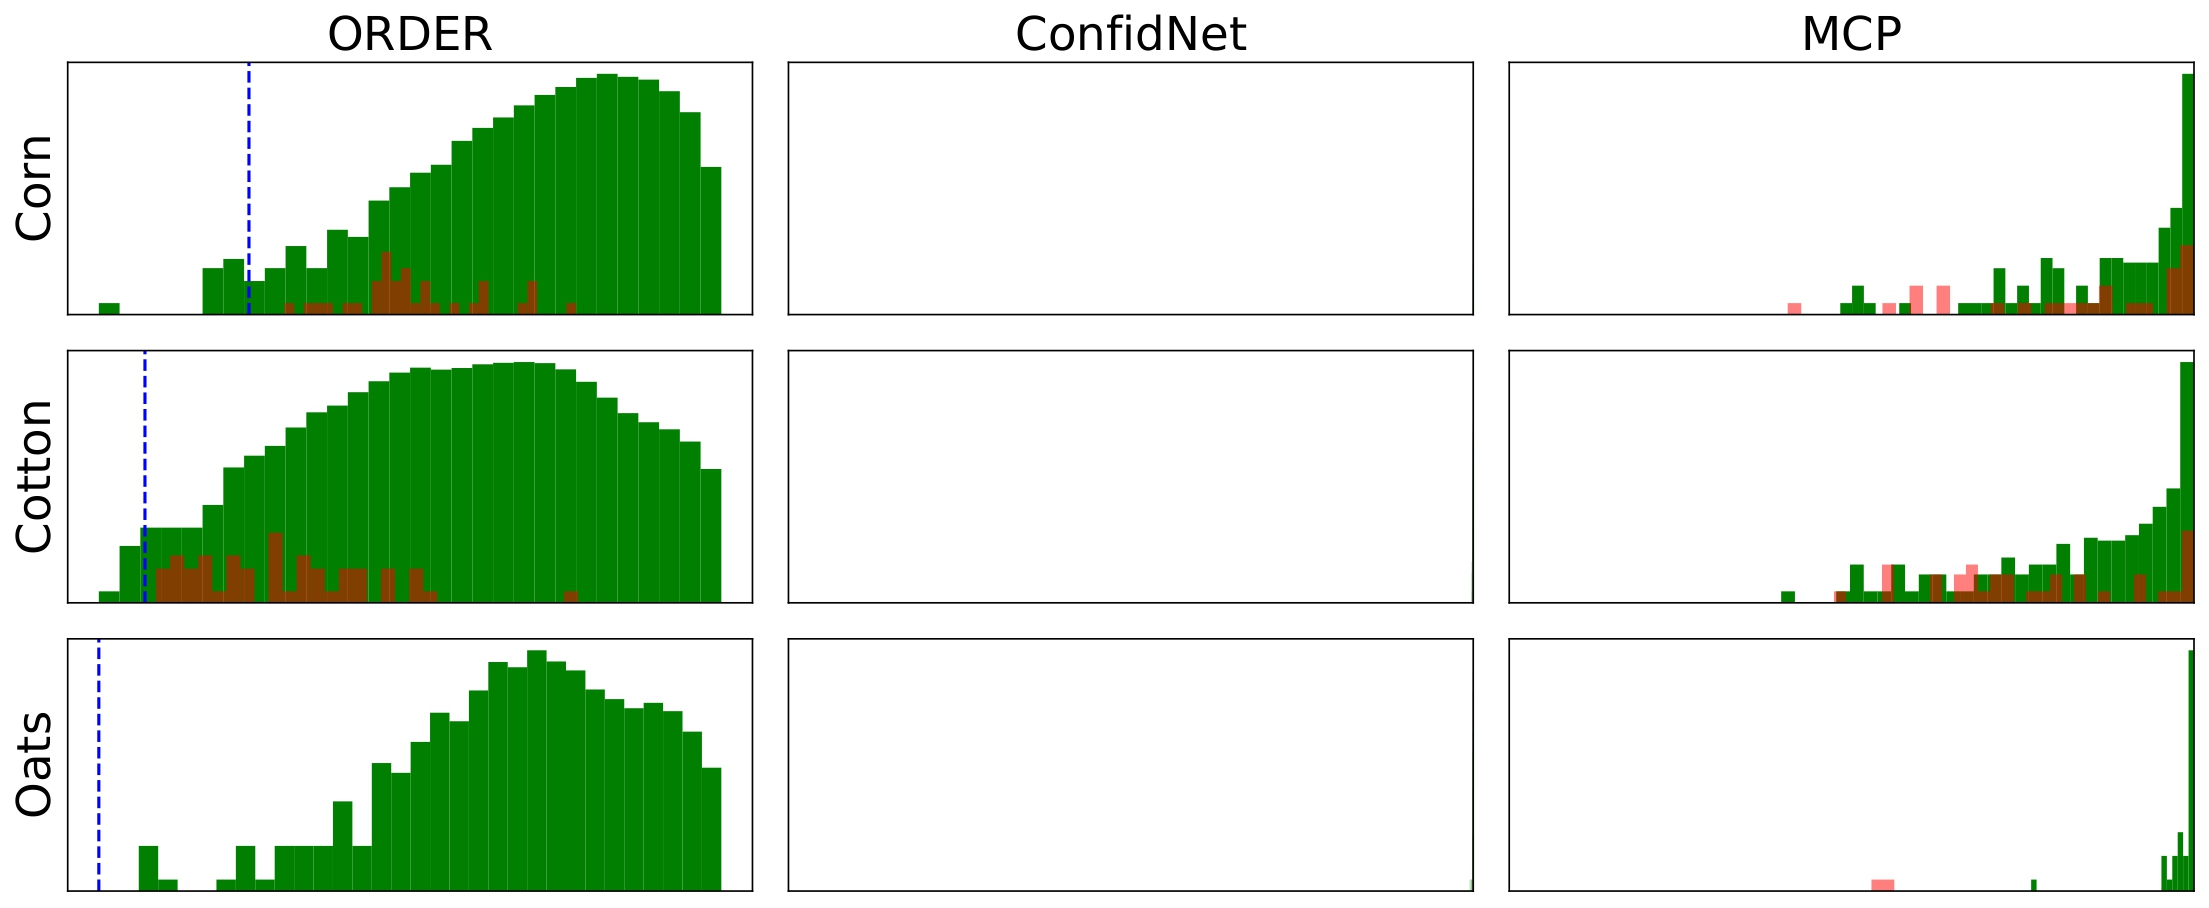
\includegraphics[height=0.41\textheight, width=\textwidth, keepaspectratio]{figures_slides/hist_combined_texas.jpg}
        % \caption*{Confusion Matrix}
    \end{figure}
\end{frame}

% --- SLIDE 8: BEST RESULT CALIFORNIA (FIGURAS 67, 68) ---

\begin{frame}{Best Setup: California Dataset}
    \begin{block}{SITS-Mamba (Masked Modeling Pre-training)}
        For the California dataset, the SITS-Mamba model leverages Masked Modeling pre-training and linear complexity to deliver highly robust performance.%, securing near-perfect predictions for Almonds and Citrus.
    \end{block}
    
    \vspace{0.2cm}
    
    \begin{columns}[T]
        \begin{column}{0.48\textwidth}
            \begin{figure}
                \centering
                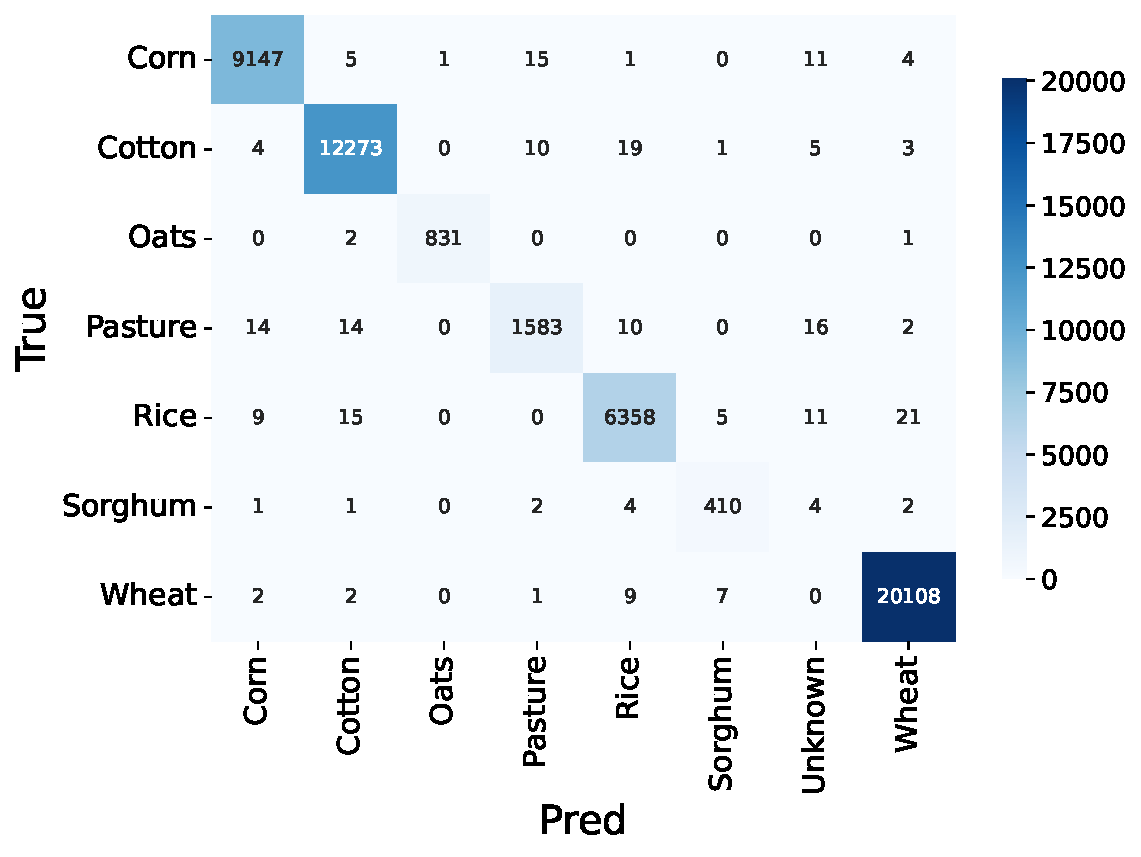
\includegraphics[height=0.45\textheight, width=\textwidth, keepaspectratio]{figures/8_results/texas-finetuning/LSTM-70.0-FastSiam/class_test_gemmos_matrix.pdf}
                % \caption*{Confusion Matrix}
            \end{figure}
        \end{column}
        \begin{column}{0.52\textwidth}
            \begin{figure}
                \centering
                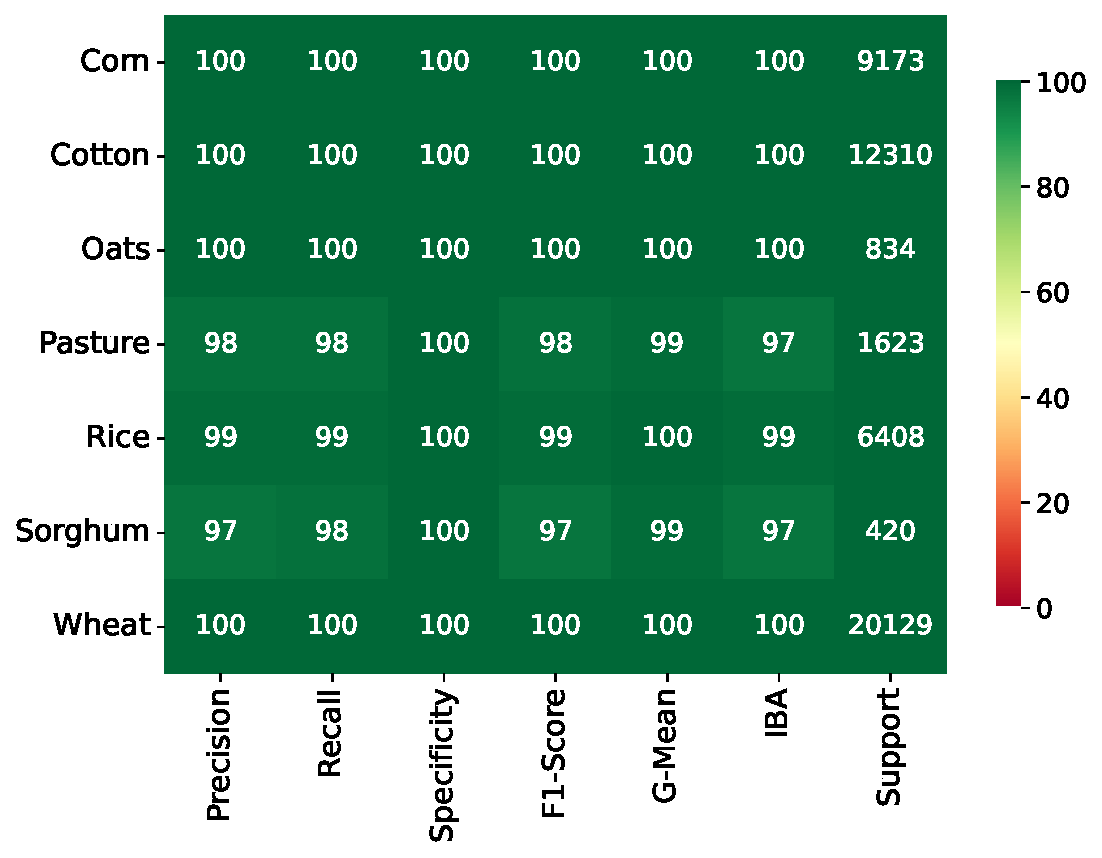
\includegraphics[height=0.45\textheight, width=\textwidth, keepaspectratio]{figures/8_results/texas-finetuning/LSTM-70.0-FastSiam/class_test_gemmos_report.pdf}
                %\caption*{Confidence Estimation (Log Scale)}
            \end{figure}
        \end{column}
    \end{columns}
\end{frame}

\begin{frame}{Best Setup: California Dataset}
    \begin{block}{SITS-Mamba (Masked Modeling Pre-training)}
        Similar to the Texas dataset, the results in California show unsaturated ORDER scores.
    \end{block}
    
    \vspace{0.2cm}
    
    \begin{figure}
        \centering
        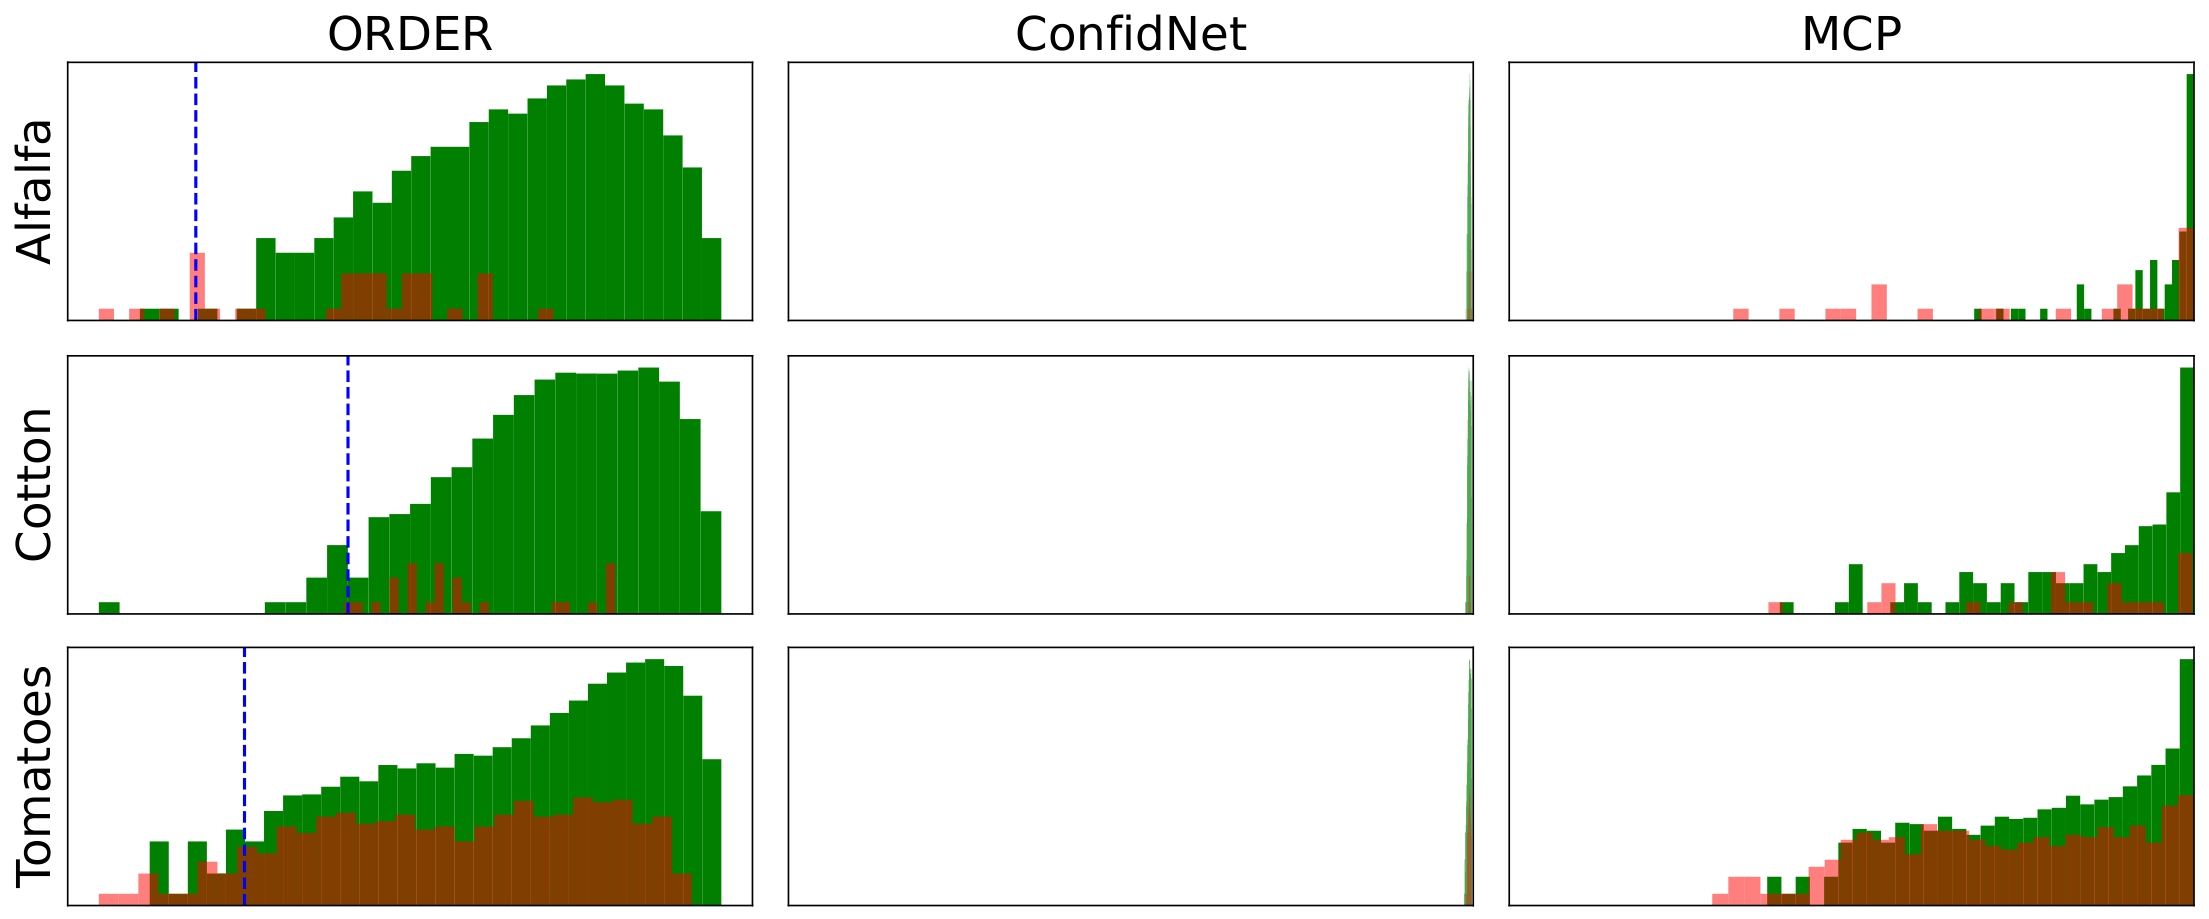
\includegraphics[height=0.41\textheight, width=\textwidth, keepaspectratio]{figures_slides/hist_combined_california.jpg}
        \caption*{Confidence Estimation (Log Scale)}
    \end{figure}
\end{frame}


